% res_steady.tex -- Results 4.1 (cont.): the steady payload error, rig and twin.
% 17 Oct (v3_full): rewritten around the measured rod pull after the appendix re-fly on the freeze tree
% (docs/analysis/appendix_refly_2026-10-17.md: C-X1, C-X2, C-D1, C-D4, C-R1-R4 confirmed; C-D2, C-D3, C-D5 falsified;
% C-G1, C-G2 unresolved; the reviewer's must-not-say list honoured: no 8.4 cm, no "learns the push" vertically, no
% 0.76 N as learned, no geometric explanation of +17.1 cm, the +13 cm box offset is not a tracking error, no "the model
% integral fails on the thrust-map error", the mass result always with the measured pull and the rigid-rod twin) and
% the exploratory cable_source model pair (R2084-R2087: push -7.95 cm, +20 % mass +22.2 cm). Rig sources unchanged:
% registry RIG-1001-*, RIG-1007-r0001/r002/r20004 (fig:rig_integral), docs/rig_2026-09-30_review.md.

\subsubsection{Steady payload error}
\label{sec:res_steady}

This part of RQ1 asks what leaves a steady error in the payload's position and what removes it, each source against
the same flight without its remedy; the bar is the ring back within 1\,cm of its target.

\paragraph{On the rig: the model integral and the measured rod pull}
\label{sec:res_rig_integral}
% Rig 7 Oct: RIG-1007-r0001 (no integral), r002 (model integral, planned pull), r20004 (model integral +
% measured pull); planner log.csv; figure tools/thesis_rig_figures.py rig_integral.

On 7 October the rig flew three hovers at 1.0\,m with four UAVs, changing one thing at a time
(Figure~\ref{fig:rig_integral}). Without an integral the ring sank in the 5\,s it held before LAND. The model
integral brought it back to its target by learning a downward force of up to 0.9\,N, but the ring then bobbed
at about 0.2\,Hz. With the trackers' measured rod pull added (Section~\ref{sec:tracker}) it held within 2\,cm
and the integral learned only 0.1\,N: most of the missing force was in the rods' pull, which the planned pull
got wrong. On the circle and the figure-eight, the measured pull with the rods planned at 60$^\circ$ cut the
standard deviation of the ring's height from 4.8--4.9 to 0.5--0.6\,cm (Table~\ref{tab:T7}). Each is one run; the
measured-pull hover held for 7\,s, ending before the first swing of the integral-only run, so the circle and the
figure-eight, flown for 36 and 68\,s, carry the claim that the swing is gone.

\begin{figure}[htbp]
\centering
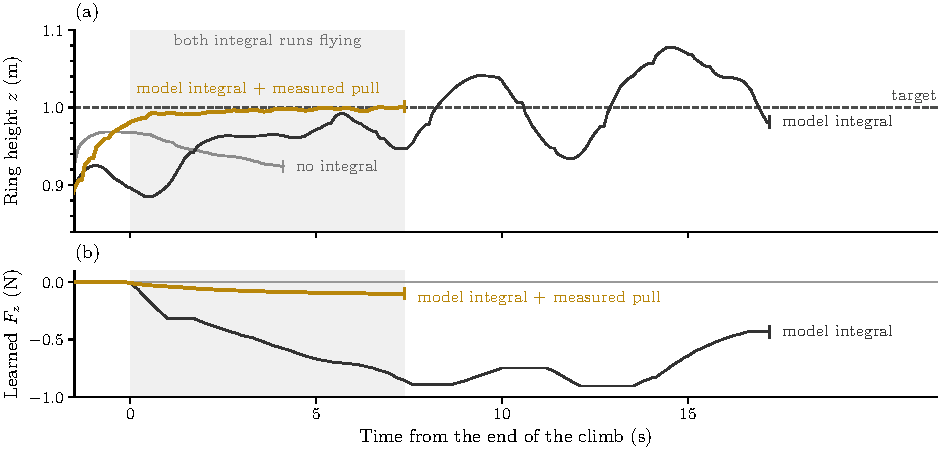
\includegraphics[width=\textwidth]{Images/rig_integral.pdf}
\caption[The model integral and the measured pull on the rig]{Ring height on the rig in a hover at 1.0\,m with
four UAVs, one change at a time (7 October, one run each; ticks: LAND). (a) Without an integral the ring sank; with the
model integral it came back but bobbed at about 0.2\,Hz; with the integral and the trackers' measured rod pull it held
between 0.98 and 1.00\,m. (b) The vertical force the integral learned: up to $-0.9$\,N on the planned pull, $-0.1$\,N on
the measured one; flat stretches: the integral frozen while the ring moves faster than 0.05\,m/s.}
\label{fig:rig_integral}
\end{figure}

\paragraph{External forces}
\label{sec:res_force}

In the twin a constant force was applied to the hovering ring for 15\,s: 0.6\,N downward, about the weight of a
60\,g object, and 0.4\,N horizontally (Table~\ref{tab:disturbance}). The vertical push leaves no steady offset, with or
without an integral: each tracker's measured pull takes up its share within about a second (the ring dips 1.4\,cm),
and the integral is left with nothing to remove. An exploratory pair with the trackers on the planner's pull instead, and
nothing else changed, left the ring 8.0\,cm low under the same push, which places the effect in the measured pull.
Horizontally the measured pull does not act on the ring's position, and the push leaves the ring 4.8\,cm off its
target; the model integral removes that offset, its force settling at 0.32\,N against the 0.40\,N applied
(Figure~\ref{fig:disturbance}, Appendix~\ref{sec:app_secondary}). As integral action does, it barely reduces the peak and overshoots by about as much when the push ends (5.3\,cm);
on the vertical push a doubled gain or a narrower gate made no resolvable difference (Table~\ref{tab:gain}, Appendix~\ref{sec:app_tests}).
When one UAV produces more thrust than its map assumes, neither form of the integral leaves a height or horizontal
error, and the ring hovers level (0.1$^\circ$); the trace reads as that UAV's own measured pull taking up its error,
though no one-variable pair separates it.



\begin{table}[htbp]
\centering
\caption[Disturbance rejection in the twin]{Disturbance rejection in the rig twin: three carriers in hover at 1.0\,m,
$\epsilon = 0$, two runs per cell on the freeze code tree. Displacement along the force, relative to its mean over
the 5\,s before the push; time to within 1\,cm after the onset; the change of the integral's force from its value
before the push.}
\label{tab:disturbance}
% generated by tools/thesis_sim_tables.py on the freeze tree (17 Oct; appendix re-fly R2027-R2033, R2039-R2045), then
% edited by hand: the planned-pull column (exploratory pair R2084, R2086, cable_source model) and footnotes a-c from
% the reviewer's corrections (docs/analysis/appendix_refly_2026-10-17.md).
\footnotesize
\setlength{\tabcolsep}{4pt}
\begin{tabular}{lcccc}
\toprule
 & \multicolumn{3}{c}{Measured rod pull} & Planned pull \\
\cmidrule(lr){2-4}\cmidrule(lr){5-5}
 & No integral & Target shift & Model integral & No integral$^c$ \\
\midrule
\multicolumn{5}{l}{\emph{0.6\,N downward push on the ring}} \\
\quad steady displacement (cm) & 0.0 (2) & 0.0 (2) & 0.0 (2) & 8.0 (2) \\
\quad peak displacement (cm) & 1.4 (2) & 1.3 (2) & 1.3 (2) & -- \\
\quad overshoot after release (cm) & 1.4 (2) & 1.5 (2) & 1.4 (2) & -- \\
\quad time to within 1\,cm (s) & 1.1 (2) & 1.0 (2) & 1.1 (2) & -- \\
\quad change of the integral force (N) & -- & -- & 0.10$^a$ (2) & -- \\
\midrule
\multicolumn{5}{l}{\emph{0.4\,N horizontal push on the ring}} \\
\quad steady displacement (cm) & 4.8 (2) & n/a & 0.0 (2) & -- \\
\quad peak displacement (cm) & 5.4 (2) & n/a & 5.5 (2) & -- \\
\quad overshoot after release (cm) & 0.7 (2) & n/a & 5.3 (2) & -- \\
\quad time to within 1\,cm (s) & -- & n/a & 4.9 (2) & -- \\
\quad change of the integral force (N) & -- & n/a & 0.32 (2) & -- \\
\midrule
\multicolumn{5}{l}{\emph{One UAV producing more thrust than its map assumes$^b$}} \\
\quad height error (cm) & -- & 0.0 (2) & $-$0.1 (2) & -- \\
\quad horizontal error (cm) & -- & 0.0 (2) & 0.0 (2) & -- \\
\quad ring tilt (\si{\degree}) & -- & 0.1 (2) & 0.1 (2) & -- \\
\bottomrule
\multicolumn{5}{p{0.95\textwidth}}{\footnotesize $^a$\,Not a learned force: it doubles with the integral gain
(0.21--0.22\,N at $k_i = 0.8$) and drifts by $-0.05$\,N with no push; the measured pull has already taken the push
up. $^b$\,Its real throttle offset 0.03 below the 0.185 its tracker assumes. $^c$\,Exploratory pair: the trackers on
the planner's pull, everything else as the first column, flown on a later code tree whose flight code differs only by
switches that are off.}
\end{tabular}

\end{table}

\paragraph{Other sources.}
\label{sec:sim_robustness}
\label{sec:res_ic}
\label{sec:res_cap}
\label{sec:res_tilt}
With one wrong value in the controller's model while the twin keeps the true one (Table~\ref{tab:robust},
Appendix~\ref{sec:app_robust}), a payload mass typed 20\,\% high or low leaves the hover where it was, with or without
the integral, because the measured pull carries what the ring actually weighs; on the planner's pull the same $+20$\,\%
left the ring 22.2\,cm high (exploratory pair), so this is a result of the rigid-rod twin on the measured pull, not a
licence to type the mass loosely. Rods typed 5\,cm long are absorbed when measured at the hand-over and leave the ring
17.1\,cm high when not, with the integral's tautness gate closed. A radius typed 2\,cm large leaves the ring 0.9\,cm high
while the vertical integral winds up without effect (0.76\,N by LAND, not a learned force). Two sources are not forces
at all. The tracker's relaxed initial condition holds the ring 13\,cm high in the twin, an offset already in the
references the planner sends, not a tracking error, and pinning node~0 removes it (Table~\ref{tab:x0}, Appendix~\ref{sec:app_tests}). The breakaway cap,
held for the whole flight on the rig on 1 October, told the trackers the rods pulled 7--27\,\% less than they did and
left the ring 20--30\,cm low until the integral took over (Appendix~\ref{sec:app_rig}); since 7 October the cap is
released at the lift. On the rig the ring also sat
3--17\,cm towards the room's $-x$ on 1 October, a force of 0.41--0.52\,N that kept its direction when the system was
rotated, and its tilt fell from 5.0$^\circ$ at 0.45\,m to 1.6$^\circ$ at 0.94\,m, close to the floor's downwash.

\paragraph{Sources of steady error}

Table~\ref{tab:error_sources} collects the sources found, how each shows at the payload and what removes it. The
approaches to model error flown on the earlier stack (a force balance, an offset-free observer, the measured cable
force, a thrust-gain trim, the rods' mass in the planner) are recorded in Appendix~\ref{sec:app_methods}; the measured
cable force is the one that became the default.

\begin{table}[htbp]
\centering
\footnotesize
\caption{Sources of steady payload error found in this work, how each shows at the payload and what
removes it, on the current controller.}
\label{tab:error_sources}
\begin{tabularx}{\textwidth}{>{\raggedright\arraybackslash}p{3.4cm}>{\raggedright\arraybackslash}X>{\raggedright\arraybackslash}p{3.6cm}}
\toprule
Source & Signature at the payload & Remedy \\
\midrule
Tracker's relaxed initial condition & held high (13\,cm, twin); in the references, not a force & pin node~0 \\
Breakaway cap held all flight & held low, rods steep (rig) & release the cap at the lift \\
Vertical force on the ring & none on the measured pull; 8\,cm for 0.6\,N on the planned pull (exploratory) & the measured rod pull \\
Horizontal force (push, wind, the rig's $-x$ pull) & a steady offset (4.8\,cm for 0.4\,N) & the model integral \\
Payload mass typed wrong & none on the measured pull (rigid-rod twin); 22\,cm for $+20$\,\% on the planned pull (exploratory) & the measured rod pull \\
Rods typed long, unmeasured & held high (17\,cm for $+5$\,cm), integral gated off & measure at the hand-over \\
Radius typed wrong & 0.9\,cm for $+2$\,cm; the vertical integral winds up & none yet \\
One UAV's thrust map wrong & none in hover on the measured pull & that UAV's measured pull \\
\bottomrule
\end{tabularx}
\end{table}

\paragraph{Answer to RQ1, steady errors.} The measured rod pull, not the integral, is what holds the ring's height on
this controller: in the rigid-rod twin it takes up a vertical push and an error in the typed payload mass at the UAVs
themselves (separated by an exploratory one-variable pair) and, on the trace, one UAV's thrust-map error; on the rig it
removed most of the force the integral had been learning.
The model integral is left with horizontal forces, which it removes, and its vertical part can wind up on an error it
cannot see. The two sources that are not forces, the tracker's relaxed initial condition and the breakaway cap, are
removed at their source, and rods typed long must be measured at the hand-over.
